\documentclass[a4paper,14pt]{extarticle}
\usepackage{fontspec}
\usepackage{polyglossia}
\setmainlanguage{russian}
\setmainfont{Times New Roman}
\setmonofont{Courier New}
\newfontfamily\cyrillicfonttt{Times New Roman}
\usepackage{geometry}
\geometry{left=2.5cm,right=1.5cm,top=2cm,bottom=2cm}
\usepackage{setspace}
\onehalfspacing
\usepackage{graphicx}
\usepackage{float}
\usepackage{caption}
\usepackage{enumitem}
\usepackage{booktabs}
\usepackage{longtable}
\usepackage{array}
\usepackage{hyperref}
\usepackage{fvextra}
\usepackage{xcolor}
\setlist{nosep,leftmargin=1.5em}
\captionsetup{font=small,skip=6pt}
\hypersetup{
colorlinks=true,
linkcolor=black,
urlcolor=blue,
pdftitle={Лабораторная работа 4. Подсказка в экранной таблице}
}
\fvset{baselinestretch=0.9,commandchars=none}
\RecustomVerbatimEnvironment{Verbatim}{Verbatim}{breaklines,breakanywhere,fontsize=\scriptsize}
\begin{document}
\begin{titlepage}
\centering
\vspace*{2.5cm}
{\Large Лабораторная работа №\,4}\\[10pt]
по дисциплине\\
«Технологии промышленной разработки программного обеспечения.\\
Основные понятия»\\[18pt]
{\large Подсказка в экранной таблице}\\[56pt]
\begin{flushleft}
\hspace{0.42\textwidth}
\begin{tabular}{ll}
Выполнил: & студент группы М26-504\\[8pt]
& Гришанов Николай Вадимович\\
\end{tabular}
\end{flushleft}
\vfill
Москва --- 2026
\end{titlepage}
\tableofcontents
\newpage
\section{Описание работы}
\subsection{Цель и постановка}
Цель работы --- разработать типовое решение подсказки для экранной таблицы Windows Forms. Подсказка отличается от штатного выпадающего списка тем, что её состав расширяется во время работы: строка, введённая в ячейку и отсутствующая в списке, становится новой строкой подсказки.
По методическим указаниям на форме стоят две таблицы \texttt{DataGridView}. Рабочая таблица \texttt{dataGridView2} содержит столбцы NN, «Название» и «Тип». Столбец «Тип» --- штатный \texttt{ComboBoxColumn} со значениями «Зверь», «Птица», «Рыба», «Гад». Вторая таблица, \texttt{dgwNamesPrompt}, скрыта до редактирования и служит окном подсказки: без заголовков столбцов и строк. Список подсказки --- \texttt{List<Names>} с одним свойством \texttt{Name}, привязанный через \texttt{BindingSource}. Меню содержит команды «Создать список», «Подключить список» и «Упорядочить».
Универсальная подсказка покрывает такие прецеденты:
\begin{enumerate}
\item после первой литеры или повторного щелчка по уже выделенной ячейке подсказка открывается, ячейка остаётся в режиме редактирования;
\item литеры попадают в ячейку, а выделение в подсказке сдвигается по возрастанию к строке, которая не меньше введённого текста;
\item стрелки вверх и вниз двигают выделение, Enter переносит выбранную строку в ячейку, Escape отказывается от подсказки;
\item Enter по набранному тексту, которого в списке нет, копирует его в подсказку, сортирует список и оставляет подсказку открытой;
\item щелчок левой кнопкой по строке подсказки копирует её в ячейку;
\item подсказка работает для любого столбца рабочей таблицы, а не только для столбца «Название».
\end{enumerate}
\subsection{Недостатки базового образца}
Текст методички задаёт класс \texttt{Prompt} и обработчики формы, но в приложенном коде сценарии расходятся с реализацией.
\begin{itemize}
\item Подсказка открывается только при \texttt{ColumnIndex == 1}. Остальные столбцы остаются без неё, хотя пункт 3.7 требует подсказку к любому столбцу.
\item \texttt{OpenPrompt} обращается к \texttt{Rows[0]} сразу после открытия. Пустой список даёт исключение, хотя сценарии 1--2 как раз начинаются с пустой подсказки.
\item Обработчики мыши и клавиатуры подписываются при каждом открытии. \texttt{ClosePrompt} снимает их только когда \texttt{Active} ложно, поэтому при наведении указателя подсказка не закрывается и подписки копятся.
\item В \texttt{Spec\_PreKeyDown} перенос строки из подсказки в ячейку завязан на Alt+Enter. В постановке выбор выполняется стрелками и обычным Enter.
\item Продвижение селекции в \texttt{Spec\_KeyPress} идёт только вперёд по \texttt{CurPromptrow}. Стирание символа не возвращает выделение к более ранней строке.
\item «Упорядочить» и \texttt{StoreNewCellValue} подменяют источник привязки новым списком и не обновляют поле \texttt{vns}. Следующее пополнение и команда меню работают уже с другим объектом.
\item «Подключить список» вызывает \texttt{Rows.Clear()} у таблицы, которая может быть уже привязана к данным. Для привязанного \texttt{DataGridView} это исключение.
\item Штатный \texttt{ComboBoxColumn} не принимает значение, которого нет в \texttt{Items}. Новая строка подсказки в столбце «Тип» без дописывания в список столбца завершается ошибкой данных.
\end{itemize}
\subsection{Принятое решение}
Окно и класс подсказки оставлены в одном модуле \texttt{Form1.cs}, как в приложении к методичке: пространство имён \texttt{TipTop}, таблица \texttt{dataGridView2}, окно \texttt{dgwNamesPrompt}, статус \texttt{toolStripStatusLabel2}. Исправлено то, что мешало прецедентам, и подсказка обобщена на все столбцы.
У каждого столбца свой \texttt{List<Names>} и свой \texttt{BindingSource}. Для столбца «Название» (индекс 1) это общие \texttt{Form1.vns} и \texttt{Form1.vbs}, поэтому три команды меню по-прежнему управляют именно этим списком. Столбцы NN и «Тип» копят собственные строки. При первом открытии столбца «Тип» в его список копируются четыре значения комбинированного столбца.
Подсказка ставится под текущую ячейку и поднимается над таблицей. Если снизу не хватает места, она открывается над ячейкой. Пока строк не больше восьми, полоса прокрутки скрыта и видны все элементы. Пустой список показывает компактное пустое окно, а не обращение к несуществующей строке.
Клавиатура обрабатывается на элементе редактирования. \texttt{PreviewKeyDown} помечает Enter, Escape и стрелки как клавиши ввода, чтобы таблица не уводила их на соседнюю ячейку. Стрелка двигает выделение подсказки. Следующий Enter переносит выделенную строку в ячейку и завершает редактирование. Enter без предварительных стрелок заносит набранный текст в список столбца, сортирует его и оставляет ячейку в редактировании. Пустой Enter завершает редактирование и оставляет подсказку на экране. Escape возвращает прежнее значение ячейки и прячет подсказку.
Щелчок по строке подсказки запоминается в \texttt{MouseDown} и применяется после текущего сообщения мыши: так значение успевает попасть в ячейку и не теряется из-за потери фокуса редактором. Пока указатель над подсказкой, флаг \texttt{Active} не даёт \texttt{CellEndEdit} закрыть окно раньше щелчка.
Новая непустая строка добавляется, только если такой ещё нет. Список заново сортируется культурой текущей локали, той же, которой пользуется \texttt{OrderBy}. Для комбинированного столбца то же значение добавляется в \texttt{Items}, поэтому ячейка «Тип» принимает введённое слово. Поиск селекции при наборе каждый раз начинается с первой строки, поэтому Backspace сдвигает выделение назад.
\section{Код}
Решение --- один проект Windows Forms SDK-стиля на .NET 10, пространство имён \texttt{TipTop}. Файл решения: \texttt{TipTop/TipTop.sln} (рядом лежит \texttt{TipTop.slnx}).
\subsection{Точка входа}
\VerbatimInput[breaklines,breakanywhere,fontsize=\scriptsize,frame=single]{../TipTop/Program.cs}
\subsection{Форма, список и подсказка}
\VerbatimInput[breaklines,breakanywhere,fontsize=\scriptsize,frame=single]{../TipTop/Form1.cs}
\subsection{Разметка окна}
\VerbatimInput[breaklines,breakanywhere,fontsize=\scriptsize,frame=single]{../TipTop/Form1.Designer.cs}
\subsection{Съёмка сценариев}
\VerbatimInput[breaklines,breakanywhere,fontsize=\scriptsize,frame=single]{../TipTop/DemoShots.cs}
\section{Описание написанного кода}
\subsection{Form1}
Конструктор собирает три столбца и восемь пустых строк. Режим редактирования --- \texttt{EditOnKeystrokeOrF2}: первый щелчок выделяет ячейку, ввод с клавиатуры или F2 открывает редактор. Повторный щелчок по уже текущей ячейке вызывает \texttt{BeginEdit(false)} и ставит каретку в начало строки. Это сценарий щелчка левой кнопкой при уже выделенной ячейке.
«Создать список» добавляет Argon, Xenon и Cripton, не дублируя уже имеющиеся имена. «Подключить список» снимает прежнюю привязку и назначает \texttt{vbs} источником \texttt{dgwNamesPrompt}; \texttt{Rows.Clear()} вызывается только пока источника ещё нет. «Упорядочить» строит новый список по возрастанию \texttt{Name}, записывает его и в \texttt{vns}, и в \texttt{vbs}. Если в этот момент открыта подсказка столбца «Название», окно подсказки пересчитывает размер.
\texttt{GetList}, \texttt{SetList} и \texttt{GetSource} отделяют столбец 1 от остальных. \texttt{CellBeginEdit} открывает подсказку для любого столбца. \texttt{CellEndEdit} переносит значение в список, если редактирование не отменено и значение пришло не из щелчка по подсказке. Флаг \texttt{KeepOpen} оставляет окно видимым после пустого Enter. Смена текущей ячейки закрывает подсказку, когда редактирование уже закончено и текущая ячейка --- другая.
\texttt{EditingControlShowing} подключает общие обработчики и к текстовому редактору, и к \texttt{ComboBox}. У комбинированного редактора стиль \texttt{DropDown}, чтобы можно было набрать новое слово, а штатный выпадающий список в этот момент закрывается: на экране остаётся окно подсказки. Стрелка комбинированного столбца по-прежнему открывает штатный список.
\subsection{Names и Prompt}
\texttt{Names} --- одна строка подсказки, свойство \texttt{Name}. Таблица подсказки показывает его автоматически через привязку.
\texttt{OpenPrompt} запоминает ячейку, привязывает список этого столбца и включает обработчики один раз. Повторный вход в ту же или другую ячейку заново ставит окно и не накапливает подписки: \texttt{Wire} проверяет флаг \texttt{wired}. Для пустого комбинированного столбца список заполняется его \texttt{Items}.
\texttt{AdjustPrompt} переводит прямоугольник ячейки в координаты формы, ограничивает окно областью между меню и строкой состояния и при нехватке места снизу переносит его вверх. Ширина колонки подсказки --- \texttt{Fill}, поэтому строка занимает всё окно.
\texttt{Spec\_KeyPress} строит текст так, как он будет выглядеть после текущей литеры, и вызывает \texttt{Advance}. Если в редакторе есть выделение, текст сначала очищается: первая литера при входе в ячейку заменяет выделенное, как в образце. \texttt{Advance} идёт с нулевой строки, пока введённый текст больше значения строки, и выделяет первую строку, которая не меньше введённого. Пустой текст выделение снимает. \texttt{Spec\_KeyUp} для Backspace и Delete пересчитывает выделение по уже изменённому тексту.
\texttt{CommitTypedText} различает пустой Enter и Enter с текстом. Пустой ввод ставит \texttt{KeepOpen} и завершает редактирование. Непустой вызывает \texttt{StoreText}, очищает выделение подсказки и оставляет редактор открытым. \texttt{StoreText} отбрасывает пустую строку и точное повторение, сортирует список, меняет источник привязки и для комбинированного столбца добавляет пункт в \texttt{Items}.
\texttt{ApplyToCell} записывает выбранную строку в редактор, завершает редактирование и прячет подсказку. Из \texttt{MouseDown} вызов откладывается через \texttt{BeginInvoke}, чтобы не завершать редактирование внутри сообщения мыши. \texttt{CancelEditAndHide} возвращает в редактор прежнее значение ячейки, отменяет ввод и закрывает окно. Если отмена из обработчика клавиши оказывается вложенной, завершение переносится в очередь сообщений формы.
\subsection{DemoShots}
Класс прогоняет окно по тем же обработчикам, которыми пользуется оператор: команды меню, \texttt{BeginEdit}, \texttt{Spec\_KeyPress}, \texttt{Spec\_KeyDown} и \texttt{prompt\_MouseDown}. После каждого контрольного состояния \texttt{PrintWindow} сохраняет снимок окна. Каталог задаётся аргументом \texttt{--demo-out}.
\section{Описание тестовых сценариев}
Окно проверяется одним прогоном:
\begin{Verbatim}
dotnet run --project TipTop -- --demo-out=..\report\images
\end{Verbatim}
Прогон выполняется из каталога \texttt{TipTop}. Снимки лежат в \texttt{report/images} и приведены ниже. В строке состояния остаётся текст, по которому видно, какое действие только что выполнено.
Сценарии идут одной цепочкой.
\begin{enumerate}
\item старт: три столбца, пустые строки, подсказка скрыта;
\item меню: создать список, подключить его и упорядочить;
\item открытие подсказки под ячейкой «Название»: Argon, Cripton, Xenon;
\item литера \texttt{C} сдвигает выделение на Cripton;
\item стрелка вниз сдвигает выделение на Xenon, Enter переносит Xenon в ячейку и прячет подсказку;
\item в соседней ячейке набирается Neon и подтверждается Enter: строка попадает в список по алфавиту, редактирование продолжается, подсказка открыта;
\item Escape отменяет набор и прячет подсказку, уже записанный Xenon остаётся в таблице;
\item пустой Enter заканчивает редактирование и оставляет подсказку видимой;
\item щелчок по первой строке подсказки переносит Argon в текущую ячейку;
\item столбец «Тип» открывает собственный список из четырёх штатных значений;
\item слово «Насекомое» добавляется в этот список, сортируется и остаётся допустимым значением комбинированного столбца;
\item столбец NN открывает свой пустой список и не показывает названия.
\end{enumerate}
\section{Тестовые сценарии}
Ниже --- состояния окна после прогона \texttt{DemoShots}. Ожидаемый состав списка и текст ячейки совпали с фактическими.
\subsection{Старт}
Шаги: запустить приложение.\\
Ожидание: меню из трёх команд, столбцы NN, «Название» и «Тип», восемь пустых строк и строка для новой записи, подсказка скрыта, в статусе памятка по клавишам.\\
Факт: совпало, рисунок~\ref{fig:start}.
\begin{figure}[H]
\centering
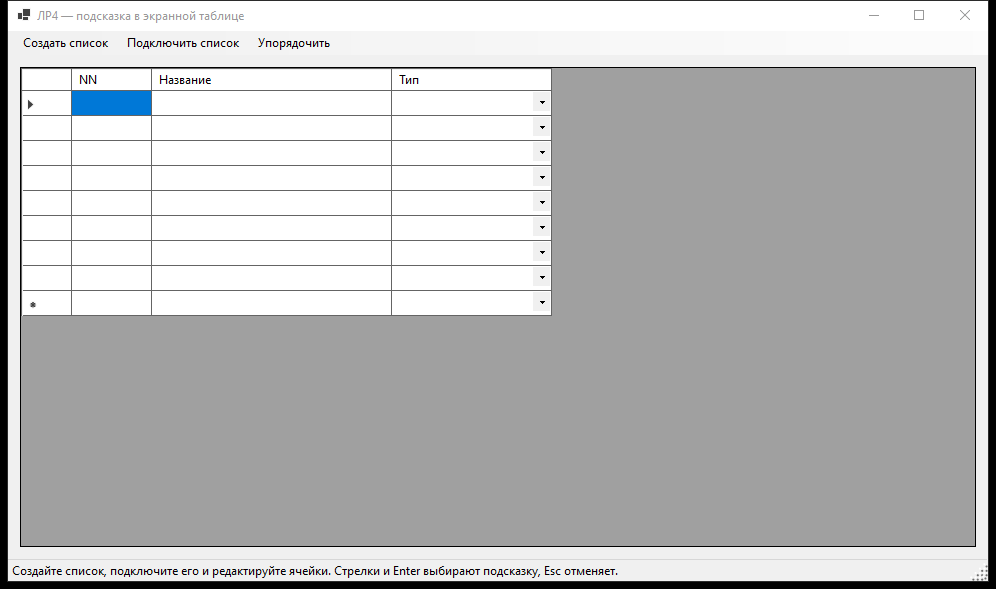
\includegraphics[width=\textwidth]{images/01-start.png}
\caption{Окно при запуске}
\label{fig:start}
\end{figure}
\subsection{Команды меню}
Шаги: «Создать список», «Подключить список», «Упорядочить».\\
Ожидание: статус «Список упорядочен». Подсказка ещё скрыта: команды только готовят список столбца «Название». Порядок имён --- Argon, Cripton, Xenon.\\
Факт: совпало, рисунок~\ref{fig:menu}.
\begin{figure}[H]
\centering
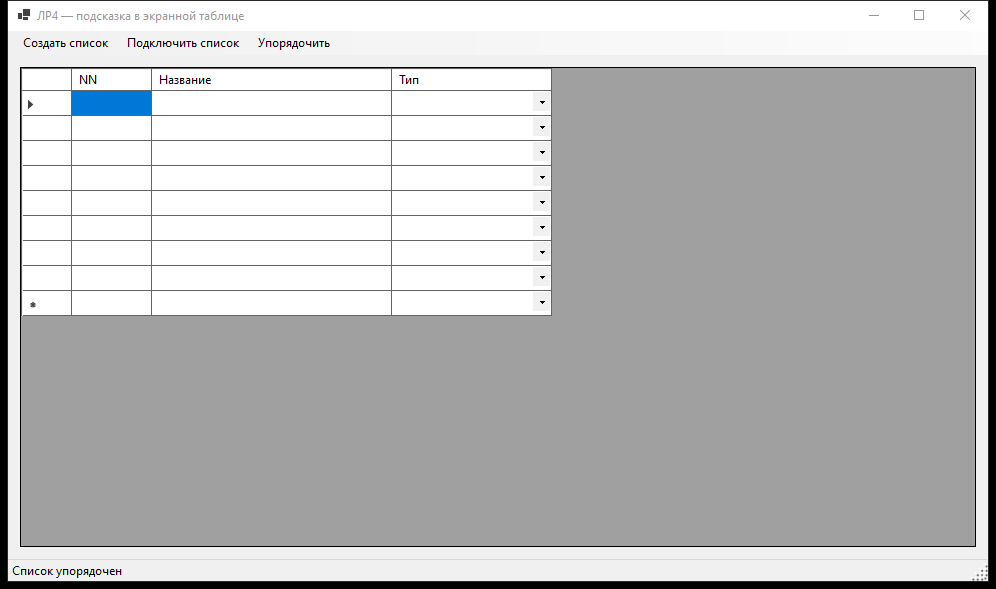
\includegraphics[width=\textwidth]{images/02-menu-sorted.png}
\caption{Список создан, подключён и упорядочен}
\label{fig:menu}
\end{figure}
\subsection{Подсказка под ячейкой «Название»}
Шаги: начать редактирование первой ячейки столбца «Название».\\
Ожидание: под ячейкой окно без заголовков, строки Argon, Cripton, Xenon, ячейка в режиме редактирования, статус сообщает, что редактор таблицы создан.\\
Факт: совпало, рисунок~\ref{fig:open}.
\begin{figure}[H]
\centering
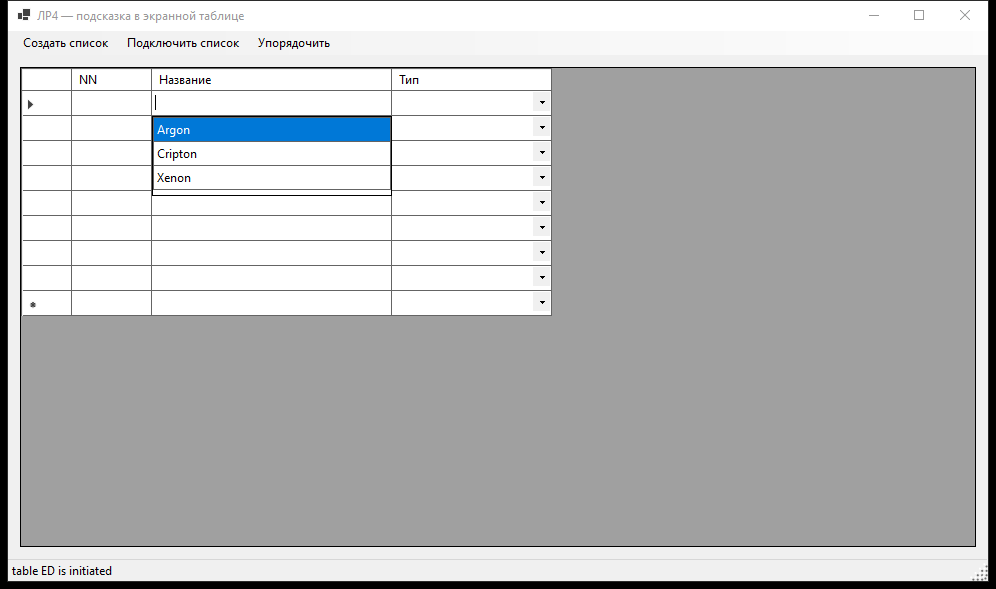
\includegraphics[width=\textwidth]{images/03-prompt-sorted.png}
\caption{Упорядоченная подсказка под столбцом «Название»}
\label{fig:open}
\end{figure}
\subsection{Продвижение селекции при вводе}
Шаги: нажать \texttt{C}.\\
Ожидание: в ячейке литера \texttt{C}, выделена первая строка, которая не меньше этого текста, --- Cripton. Argon остаётся выше, Xenon ниже.\\
Факт: совпало, рисунок~\ref{fig:typec}.
\begin{figure}[H]
\centering
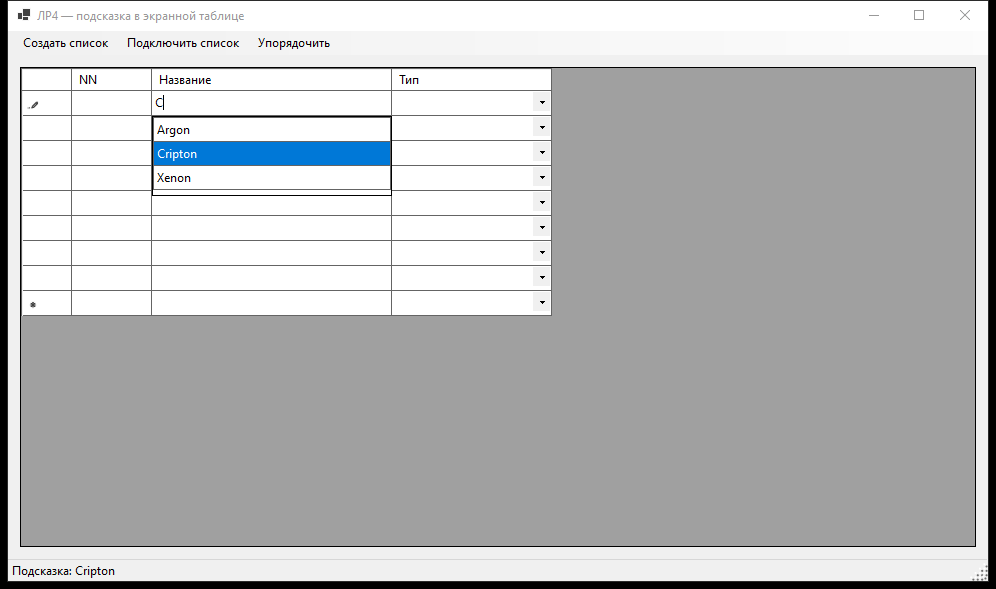
\includegraphics[width=\textwidth]{images/04-type-c.png}
\caption{После литеры \texttt{C} выделена строка Cripton}
\label{fig:typec}
\end{figure}
\subsection{Стрелка вниз}
Шаги: нажать стрелку вниз.\\
Ожидание: выделение переходит на Xenon, набранная литера \texttt{C} в ячейке сохраняется, статус показывает «Подсказка: Xenon».\\
Факт: совпало, рисунок~\ref{fig:down}.
\begin{figure}[H]
\centering
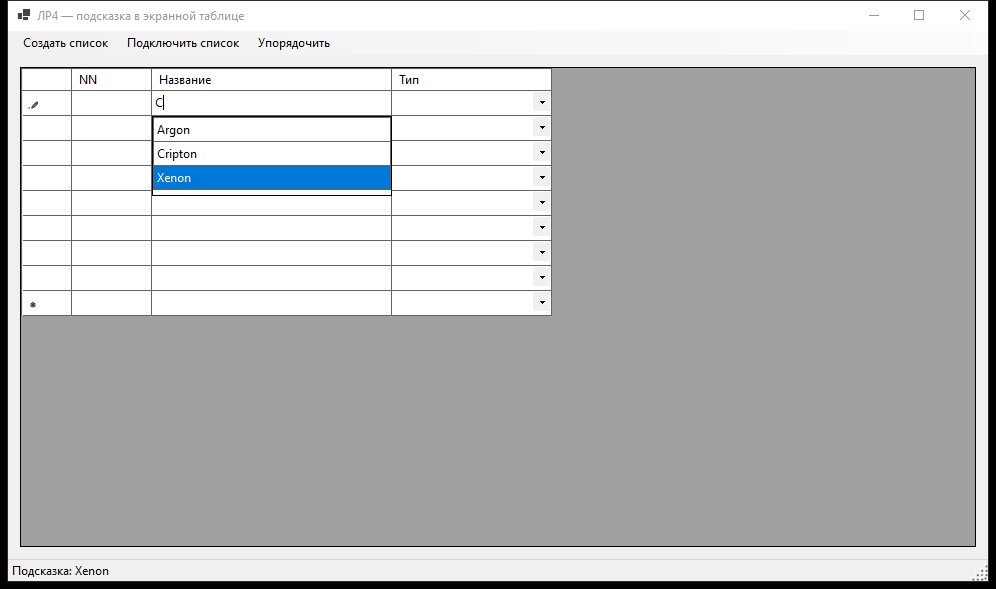
\includegraphics[width=\textwidth]{images/05-arrow-down.png}
\caption{Стрелка вниз переводит выделение на Xenon}
\label{fig:down}
\end{figure}
\subsection{Enter переносит строку подсказки}
Шаги: нажать Enter после стрелки.\\
Ожидание: в ячейке Xenon, редактирование закончено, подсказка скрыта, статус --- \texttt{write from prompt to table}.\\
Факт: совпало, рисунок~\ref{fig:enter}.
\begin{figure}[H]
\centering
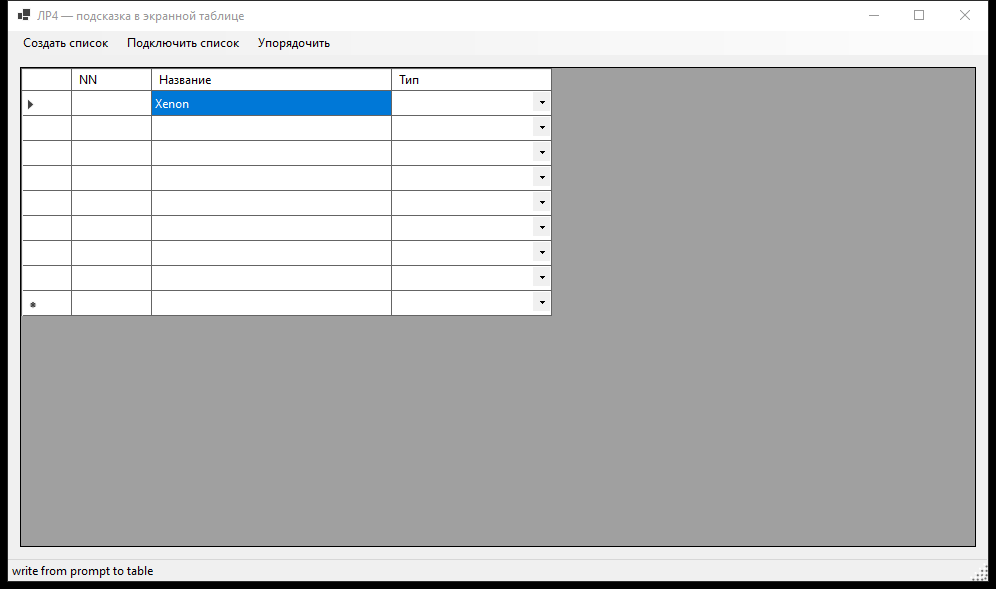
\includegraphics[width=\textwidth]{images/06-enter-hint.png}
\caption{Xenon перенесён из подсказки в ячейку}
\label{fig:enter}
\end{figure}
\subsection{Новая строка попадает в подсказку}
Шаги: открыть следующую ячейку «Название», набрать Neon, нажать Enter, не двигая выделение стрелками.\\
Ожидание: Neon остаётся в редакторе, подсказка открыта и упорядочена: Argon, Cripton, Neon, Xenon. Статус --- «Строка занесена в подсказку». Повтора Neon нет.\\
Факт: совпало, рисунок~\ref{fig:neon}.
\begin{figure}[H]
\centering
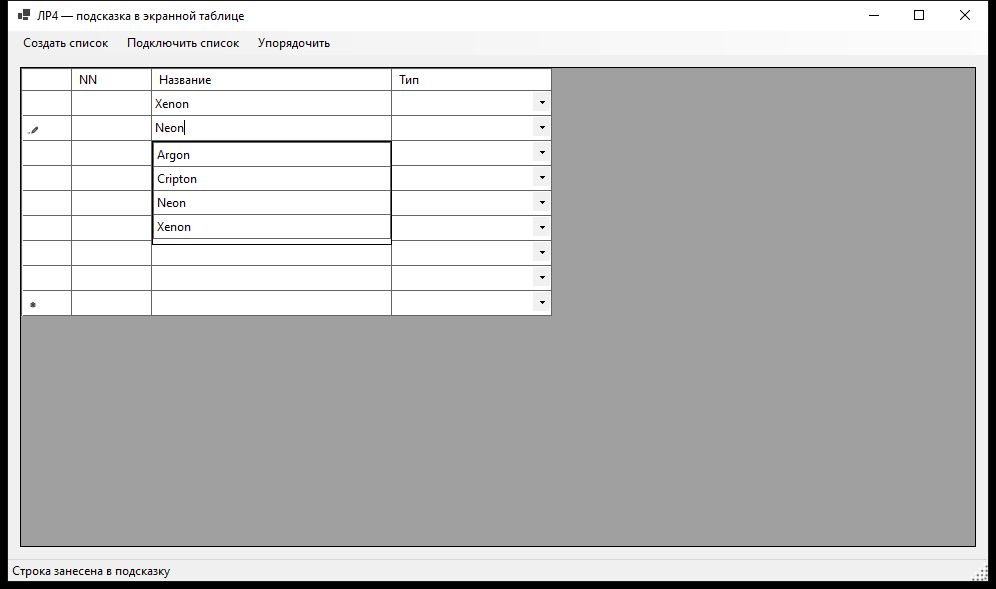
\includegraphics[width=\textwidth]{images/07-store-new.png}
\caption{Neon добавлен в список и стоит между Cripton и Xenon}
\label{fig:neon}
\end{figure}
\subsection{Отказ по Escape}
Шаги: при открытой подсказке нажать Escape.\\
Ожидание: редактирование прекращено, набранный текст в ячейку не записывается, подсказка скрыта. Xenon в первой строке на месте. Статус --- «Подсказка скрыта».\\
Факт: совпало, рисунок~\ref{fig:esc}.
\begin{figure}[H]
\centering
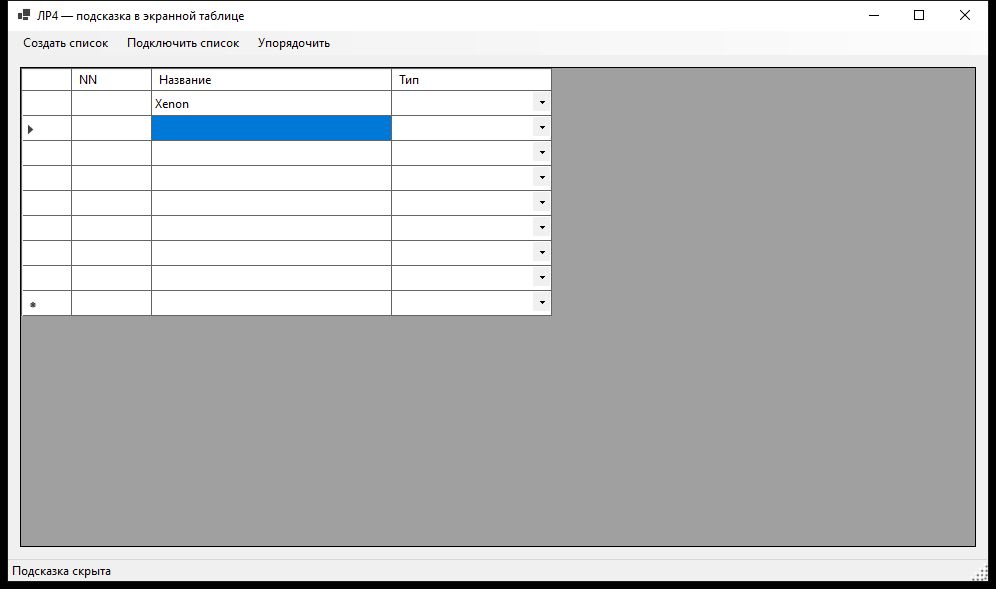
\includegraphics[width=\textwidth]{images/08-escape.png}
\caption{Escape скрыл подсказку и не записал черновик}
\label{fig:esc}
\end{figure}
\subsection{Пустой Enter оставляет подсказку}
Шаги: открыть пустую ячейку «Название» и нажать Enter.\\
Ожидание: редактирование закончено, подсказка остаётся под ячейкой и показывает уже накопленный список, включая Neon. Статус --- «Ячейка закрыта, подсказка видима».\\
Факт: совпало, рисунок~\ref{fig:empty}.
\begin{figure}[H]
\centering
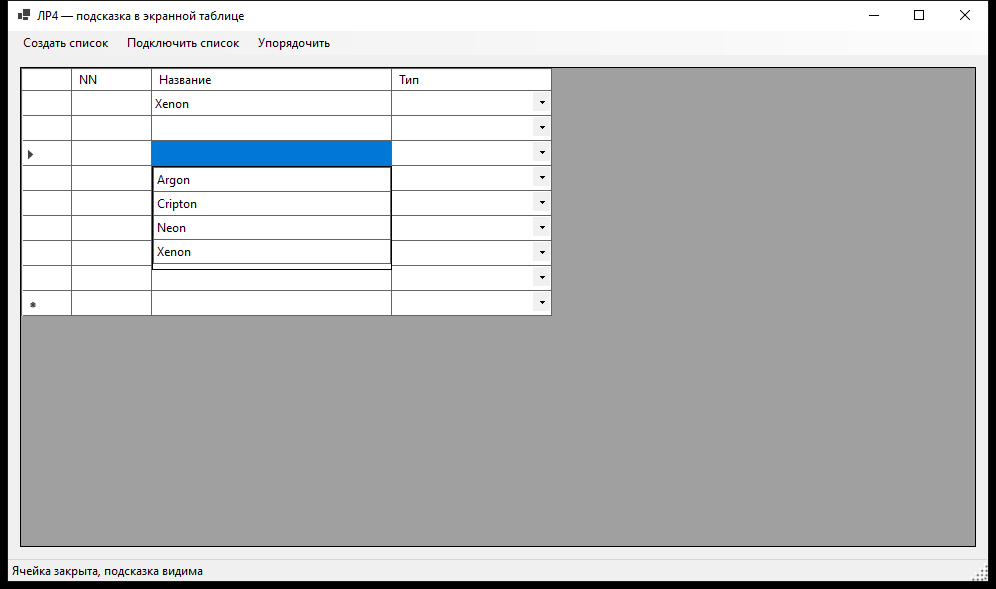
\includegraphics[width=\textwidth]{images/09-empty-enter.png}
\caption{Пустой Enter закрыл ячейку и оставил подсказку}
\label{fig:empty}
\end{figure}
\subsection{Щелчок по строке подсказки}
Шаги: начать редактирование другой ячейки «Название» и нажать левую кнопку на первой строке подсказки.\\
Ожидание: в ячейку попадает Argon, подсказка скрывается, статус --- \texttt{write from prompt to table}.\\
Факт: совпало, рисунок~\ref{fig:mouse}.
\begin{figure}[H]
\centering
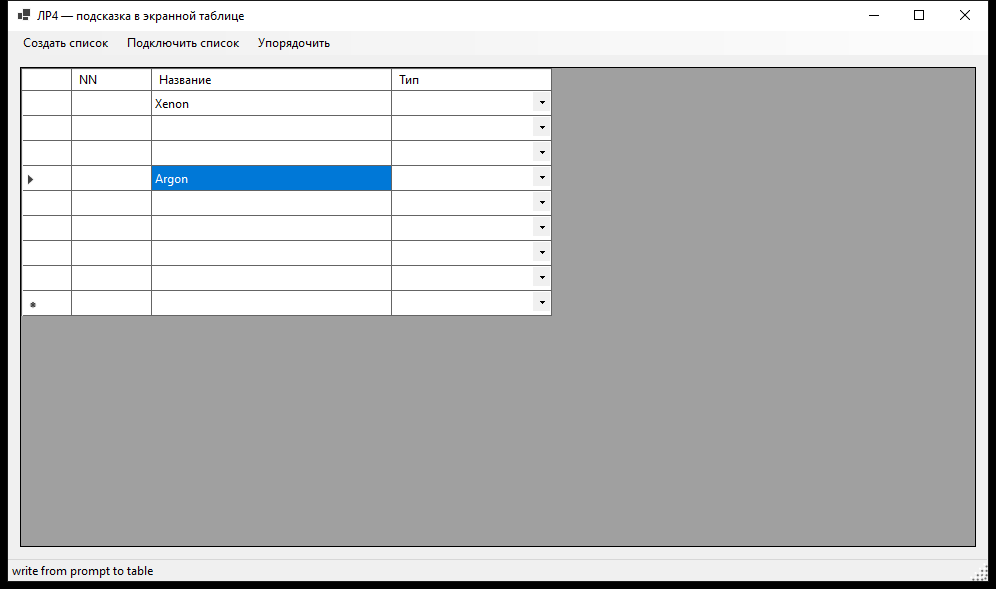
\includegraphics[width=\textwidth]{images/10-mouse.png}
\caption{Щелчок по строке Argon перенёс её в ячейку}
\label{fig:mouse}
\end{figure}
\subsection{Подсказка столбца «Тип»}
Шаги: начать редактирование ячейки «Тип».\\
Ожидание: под ячейкой собственный список из штатных пунктов комбинированного столбца: Зверь, Птица, Рыба, Гад. Список названий в это окно не попадает. Редактор допускает ввод текста.\\
Факт: совпало, рисунок~\ref{fig:type}.
\begin{figure}[H]
\centering
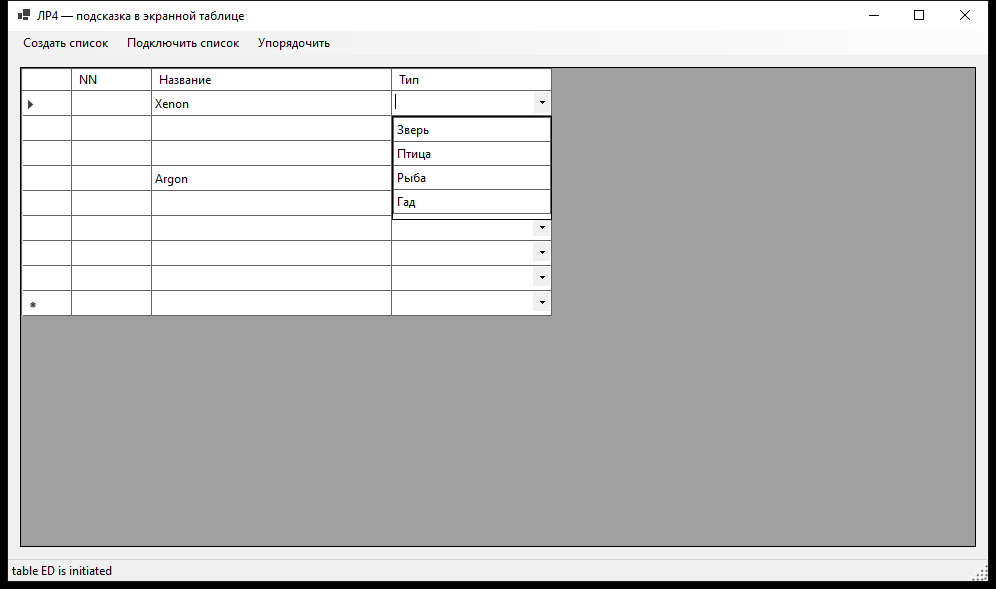
\includegraphics[width=\textwidth]{images/11-type-column.png}
\caption{Столбец «Тип» открывает свой список}
\label{fig:type}
\end{figure}
\subsection{Расширение комбинированного столбца}
Шаги: набрать «Насекомое» и нажать Enter.\\
Ожидание: слово остаётся в ячейке, подсказка столбца «Тип» упорядочена: Гад, Зверь, Насекомое, Птица, Рыба. Значение добавлено и в пункты \texttt{ComboBoxColumn}, поэтому ячейка его принимает. Статус --- «Строка занесена в подсказку».\\
Факт: совпало, рисунок~\ref{fig:insect}.
\begin{figure}[H]
\centering
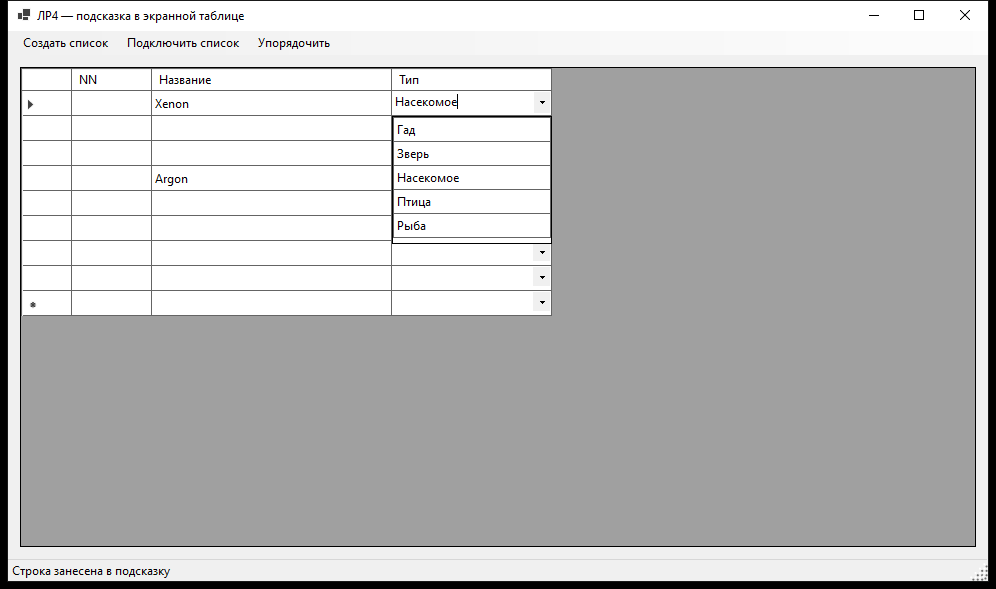
\includegraphics[width=\textwidth]{images/12-new-type.png}
\caption{«Насекомое» добавлено в подсказку столбца «Тип»}
\label{fig:insect}
\end{figure}
\subsection{Отдельный список столбца NN}
Шаги: начать редактирование ячейки NN.\\
Ожидание: под ячейкой пустое окно. Названия и типы в него не подставляются: у столбца ещё нет своих строк.\\
Факт: совпало, рисунок~\ref{fig:nn}.
\begin{figure}[H]
\centering
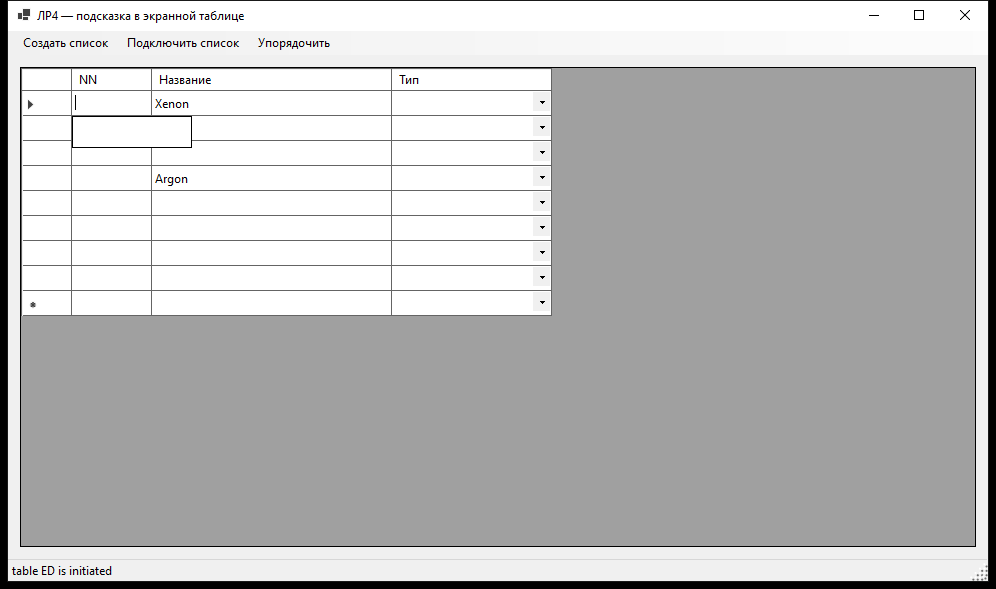
\includegraphics[width=\textwidth]{images/13-nn-column.png}
\caption{Столбец NN открывает пустую подсказку}
\label{fig:nn}
\end{figure}
\section{Документация}
\subsection{Руководство оператора}
Запуск: \texttt{dotnet run --project TipTop} из каталога лабораторной либо открытие \texttt{TipTop/TipTop.sln} и запуск из Visual Studio. Открывается одно окно.
Список для столбца «Название» готовится меню, в таком порядке: «Создать список», «Подключить список», «Упорядочить». Создать список можно и повторно: Argon, Xenon и Cripton второй раз не добавляются. «Упорядочить» сортирует только этот список. Списки NN и «Тип» команда не меняет: они сортируются сами в момент добавления новой строки.
Ячейку выделяют щелчком. Редактирование начинается со второго щелчка по ней, с клавиши F2 или с первой буквы. Подсказка появляется под ячейкой. Буквы набираются в ячейку, а выделение в списке идёт к подходящей строке. Стрелки вверх и вниз двигают это выделение, не выходя из ячейки. Enter после стрелки или щелчок по строке подсказки записывает выбранное значение и закрывает подсказку.
Enter без стрелок, если в ячейке есть текст, добавляет этот текст в подсказку текущего столбца и оставляет ячейку открытой. Пустой Enter закрывает редактирование и не прячет подсказку. Escape отменяет набранное и прячет подсказку. Переход в другую ячейку тоже прячет подсказку.
В столбце «Тип» одновременно есть штатный список и окно подсказки. Новое слово, подтверждённое Enter, в дальнейшем можно выбрать и там, и там.
\subsection{Клавиши}
\begin{center}
\begin{tabular}{p{0.32\textwidth}p{0.58\textwidth}}
\toprule
Клавиша & Действие во время редактирования\\
\midrule
буквы и другие печатные символы & ввод в ячейку и сдвиг выделения подсказки\\
стрелка вверх, стрелка вниз & предыдущая или следующая строка подсказки\\
Enter после стрелки & перенести выделенную строку в ячейку и закрыть подсказку\\
Enter с набранным текстом & занести текст в подсказку, оставить ячейку в редактировании\\
Enter в пустой ячейке & закончить редактирование, подсказку не скрывать\\
Escape & отменить ввод и скрыть подсказку\\
Backspace, Delete & стереть символ и заново найти строку подсказки\\
щелчок по строке подсказки & перенести эту строку в ячейку\\
\bottomrule
\end{tabular}
\end{center}
\subsection{Сборка}
Нужен SDK .NET 10 с поддержкой Windows Forms. Из каталога \texttt{TipTop}:
\begin{Verbatim}
dotnet build TipTop.csproj
dotnet run
\end{Verbatim}
Снимки сценариев повторно снимаются так:
\begin{Verbatim}
dotnet run -- --demo-out=..\report\images
\end{Verbatim}
Отчёт собирается XeLaTeX из каталога \texttt{report}. Нужны пакеты \texttt{polyglossia}, \texttt{fontspec}, \texttt{fvextra}, шрифты Times New Roman и Courier New:
\begin{Verbatim}
xelatex lab4_report.tex
xelatex lab4_report.tex
\end{Verbatim}
Второй проход нужен для оглавления и ссылок на рисунки.
\subsection{Ограничения}
Сравнение строк зависит от текущей локали и учитывает регистр: «argon» и «Argon» --- разные строки подсказки. Меню «Упорядочить» сортирует только список столбца «Название». Стрелки двигают выделение в окне подсказки и не переводят в него фокус, поэтому набор текста не прерывается. Enter принимает выделенную строку только после стрелки; Enter сразу после набора заносит в список сам набранный текст. Каретка остаётся в конце набора, середина строки отдельно не правится. Штатный список столбца «Тип» при начале редактирования закрывается, чтобы не закрывать окно подсказки; его открывает стрелка комбинированной ячейки. Пустая подсказка --- небольшое пустое окно, а не сообщение об ошибке.
\subsection{Состав поставки}
\begin{center}
\begin{tabular}{p{0.46\textwidth}p{0.46\textwidth}}
\toprule
Путь & Назначение\\
\midrule
\texttt{TipTop/TipTop.sln} & решение для Visual Studio\\
\texttt{TipTop/TipTop.csproj} & проект Windows Forms, .NET 10\\
\texttt{TipTop/Program.cs} & запуск окна или съёмки сценариев\\
\texttt{TipTop/Form1.cs} & форма, класс \texttt{Names}, класс \texttt{Prompt}\\
\texttt{TipTop/Form1.Designer.cs} & меню, таблицы, строка состояния\\
\texttt{TipTop/DemoShots.cs} & прогон и снимки сценариев\\
\texttt{report/lab4\_report.tex} & настоящий отчёт\\
\texttt{report/images} & снимки тринадцати сценариев\\
\bottomrule
\end{tabular}
\end{center}
\section*{Заключение}
\addcontentsline{toc}{section}{Заключение}
По методичке собрано окно с рабочей таблицей и отдельным окном подсказки. Штатный комбинированный столбец «Тип» сохранён и дополнен тем же механизмом подсказки, что и текстовые столбцы. Список ведётся отдельно для каждого столбца, пополняется новыми строками без повторов и сортируется. Выбор из подсказки выполняется стрелками и Enter либо щелчком, отказ --- клавишей Escape. Цепочка из тринадцати состояний окна снята прогоном \texttt{DemoShots}: от пустой таблицы и команд меню до переноса значения из подсказки, добавления новой строки и отдельного списка у каждого столбца.
\end{document}
